% Wed Feb 25 11:41:56 2026
% This file was created with matplot2tikz v0.5.3.
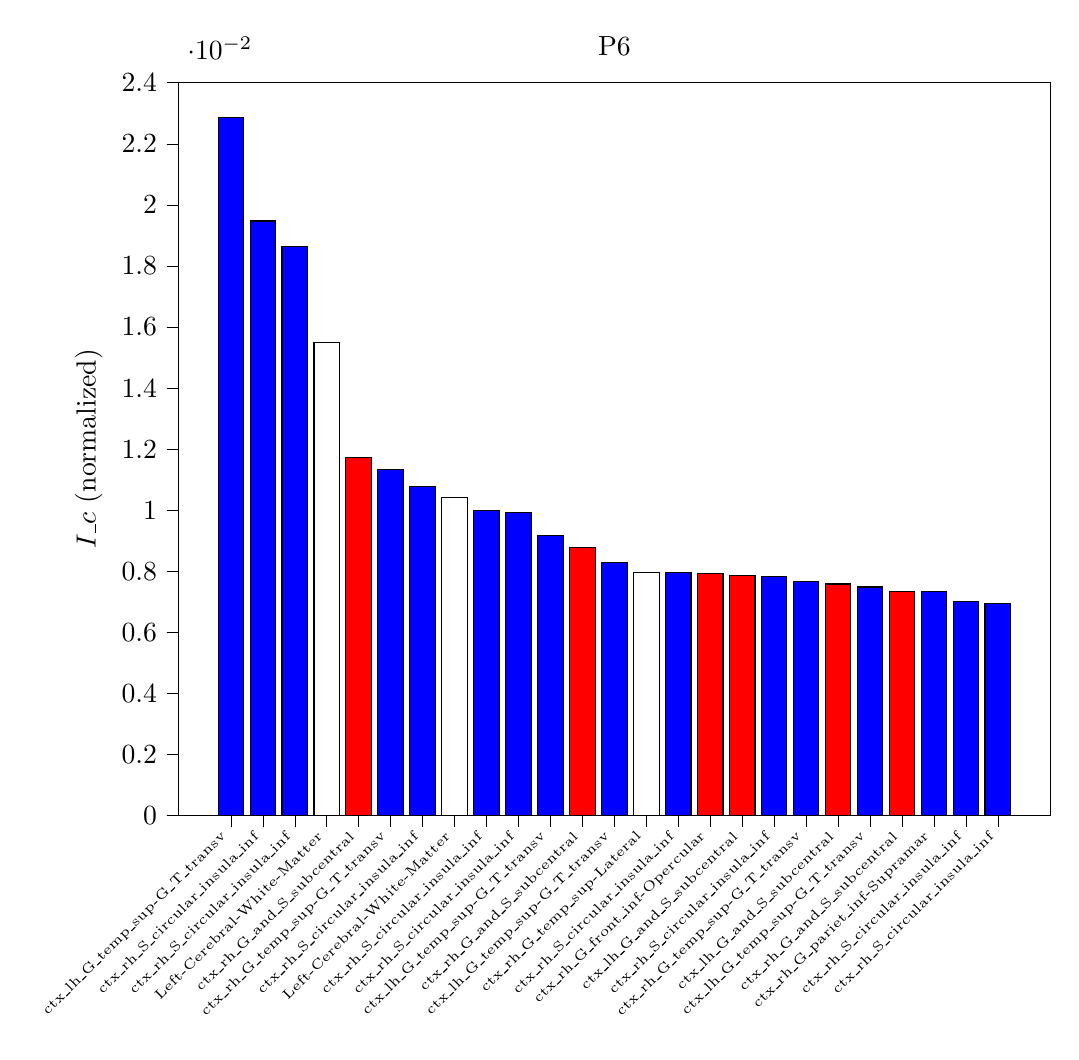
\begin{tikzpicture}
\providecommand{\thisXlabelopacity}{1.0}%
\providecommand{\figheight}{310pt}%
\provideboolean{CLEANXAXIS}\ifthenelse{\boolean{CLEANXAXIS}}{%
	\pgfplotsset{every axis post/.append style={xticklabels = {} }}%
}{}%
\providecommand{\thisYlabelopacity}{1.0}%
\providecommand{\figwidth}{360pt}%
\provideboolean{CLEARYLABEL}\ifthenelse{\boolean{CLEARYLABEL}}{%
	\pgfplotsset{every axis post/.append style={ylabel = {} }}%
}{}%
\provideboolean{CLEARXLABEL}\ifthenelse{\boolean{CLEARXLABEL}}{%
	\pgfplotsset{every axis post/.append style={xlabel = {} }}%
}{}%
\provideboolean{NOLEGEND}%
\provideboolean{CLEANXAXIS}\ifthenelse{\boolean{CLEANXAXIS}}{%
	\pgfplotsset{every axis post/.append style={xlabel = {} }}%
}{}%
\provideboolean{CLEANYAXIS}\ifthenelse{\boolean{CLEANYAXIS}}{%
	\pgfplotsset{every axis post/.append style={ylabel = {} }}%
}{}%
\provideboolean{CLEANYAXIS}\ifthenelse{\boolean{CLEANYAXIS}}{%
	\pgfplotsset{every axis post/.append style={yticklabels = {} }}%
}{}%
\pgfplotsset{compat=1.18}%
\provideboolean{CLEANTITLE}\ifthenelse{\boolean{CLEANTITLE}}{%
	\pgfplotsset{every axis post/.append style={title = {} }}%
}{}%

\definecolor{darkgray176}{RGB}{176,176,176}

\begin{axis}[
tick align=outside,
tick pos=left,
title={P6},
x grid style={darkgray176},
xmin=-1.64, xmax=25.64,
xtick style={color=black},
xtick={0,1,2,3,4,5,6,7,8,9,10,11,12,13,14,15,16,17,18,19,20,21,22,23,24},
xticklabels={
  ctx\_lh\_G\_temp\_sup-G\_T\_transv,
  ctx\_rh\_S\_circular\_insula\_inf,
  ctx\_rh\_S\_circular\_insula\_inf,
  Left-Cerebral-White-Matter,
  ctx\_rh\_G\_and\_S\_subcentral,
  ctx\_rh\_G\_temp\_sup-G\_T\_transv,
  ctx\_rh\_S\_circular\_insula\_inf,
  Left-Cerebral-White-Matter,
  ctx\_rh\_S\_circular\_insula\_inf,
  ctx\_rh\_S\_circular\_insula\_inf,
  ctx\_lh\_G\_temp\_sup-G\_T\_transv,
  ctx\_rh\_G\_and\_S\_subcentral,
  ctx\_lh\_G\_temp\_sup-G\_T\_transv,
  ctx\_rh\_G\_temp\_sup-Lateral,
  ctx\_rh\_S\_circular\_insula\_inf,
  ctx\_rh\_G\_front\_inf-Opercular,
  ctx\_lh\_G\_and\_S\_subcentral,
  ctx\_rh\_S\_circular\_insula\_inf,
  ctx\_rh\_G\_temp\_sup-G\_T\_transv,
  ctx\_lh\_G\_and\_S\_subcentral,
  ctx\_lh\_G\_temp\_sup-G\_T\_transv,
  ctx\_rh\_G\_and\_S\_subcentral,
  ctx\_rh\_G\_pariet\_inf-Supramar,
  ctx\_rh\_S\_circular\_insula\_inf,
  ctx\_rh\_S\_circular\_insula\_inf
},
y grid style={darkgray176},
ylabel={\(\displaystyle I\_c\) (normalized)},
ymin=0, ymax=0.0240189512260258,
ytick style={color=black},
every axis x label/.append style={opacity=\thisXlabelopacity},
every axis y label/.append style={opacity=\thisYlabelopacity},
height=\figheight,
width=\figwidth,
xticklabel style={rotate=45.0,anchor=east,font=\tiny}
]
\draw[draw=black,fill=blue] (axis cs:-0.4,0) rectangle (axis cs:0.4,0.0228751916438341);
\draw[draw=black,fill=blue] (axis cs:0.6,0) rectangle (axis cs:1.4,0.0194721557199955);
\draw[draw=black,fill=blue] (axis cs:1.6,0) rectangle (axis cs:2.4,0.0186337977647781);
\draw[draw=black,fill=white] (axis cs:2.6,0) rectangle (axis cs:3.4,0.0154897384345531);
\draw[draw=black,fill=red] (axis cs:3.6,0) rectangle (axis cs:4.4,0.0117218950763345);
\draw[draw=black,fill=blue] (axis cs:4.6,0) rectangle (axis cs:5.4,0.0113259851932526);
\draw[draw=black,fill=blue] (axis cs:5.6,0) rectangle (axis cs:6.4,0.0107627166435122);
\draw[draw=black,fill=white] (axis cs:6.6,0) rectangle (axis cs:7.4,0.0104108722880483);
\draw[draw=black,fill=blue] (axis cs:7.6,0) rectangle (axis cs:8.4,0.00998848676681519);
\draw[draw=black,fill=blue] (axis cs:8.6,0) rectangle (axis cs:9.4,0.0099118622019887);
\draw[draw=black,fill=blue] (axis cs:9.6,0) rectangle (axis cs:10.4,0.00916894990950823);
\draw[draw=black,fill=red] (axis cs:10.6,0) rectangle (axis cs:11.4,0.00878960825502872);
\draw[draw=black,fill=blue] (axis cs:11.6,0) rectangle (axis cs:12.4,0.00828964728862047);
\draw[draw=black,fill=white] (axis cs:12.6,0) rectangle (axis cs:13.4,0.00797025393694639);
\draw[draw=black,fill=blue] (axis cs:13.6,0) rectangle (axis cs:14.4,0.00795574299991131);
\draw[draw=black,fill=red] (axis cs:14.6,0) rectangle (axis cs:15.4,0.00793264899402857);
\draw[draw=black,fill=red] (axis cs:15.6,0) rectangle (axis cs:16.4,0.00785346888005733);
\draw[draw=black,fill=blue] (axis cs:16.6,0) rectangle (axis cs:17.4,0.00782915018498898);
\draw[draw=black,fill=blue] (axis cs:17.6,0) rectangle (axis cs:18.4,0.00766048161312938);
\draw[draw=black,fill=red] (axis cs:18.6,0) rectangle (axis cs:19.4,0.00758379558101296);
\draw[draw=black,fill=blue] (axis cs:19.6,0) rectangle (axis cs:20.4,0.00748535897582769);
\draw[draw=black,fill=red] (axis cs:20.6,0) rectangle (axis cs:21.4,0.00734147196635604);
\draw[draw=black,fill=blue] (axis cs:21.6,0) rectangle (axis cs:22.4,0.00732459221035242);
\draw[draw=black,fill=blue] (axis cs:22.6,0) rectangle (axis cs:23.4,0.00699725281447172);
\draw[draw=black,fill=blue] (axis cs:23.6,0) rectangle (axis cs:24.4,0.00695652980357409);
\ifthenelse{\boolean{NOLEGEND}}{\legend{}}{}
\end{axis}

\end{tikzpicture}
